%!TEX root = ../report.tex
%\cleardoublepage
%\clearpage
%
%\appendix
%\appendixpage
%\addappheadtotoc

\begin{appendices}
			
	%\addcontentsline{toc}{part}{\appendixname}
				
	\renewcommand{\thechapter}{\Alph{chapter}}
	\renewcommand{\thesection}{\thechapter.\arabic{section}}
	\renewcommand{\thesubsection}{\thesection.\arabic{subsection}}
	\renewcommand{\thesubsubsection}{\thesubsection.\arabic{subsubsection}}
	
	\chapter{Requirements}
	\section{Usecases}
	This section elaborates the architectural important use-cases using tables.
	
	\subsection{Receive weather/GEO/demographic data}
	\begin{table}[H]
	\pgfplotstabletypeset[%
		UCTable
	]{%
		value & description \\
		Number & \req{uc}\\
		Description & The system receives data from the weather forecast service, the geographic API and the demographic API \\
		Stakeholders and interests & 
		\textbf{Third Party}, \textbf{Safety Region} and \textbf{Citizens}: They want to receive accurate warnings about floods. \\
		Primary actor & System (timer)\\
		Scope & Monitoring part of the system \\
		Level & Sub process\\
		Precondition & There is a connection between the API and our system \\
		Main success scenario & \compactList{enumerate}{%
			\item The processing unit determines it needs external data%
			\item A call is made to the relevant external API%
			\item The external API returns the requested data
			}\\
		Postcondition & The system received the external data \\
		Alternatives & \compactList{itemize}{%
			\item[3a.] 
			\begin{enumerate}
				\item The data cannot be returned.
				\item Repeat this process with another external API service.
				\item If none are available, proceed monitoring without the requested external data.
				\item After 5 minutes try to reconnect.
			\end{enumerate}
			}\\
		Related requirements & \ref{fr:receive-weather}, \ref{fr:receive-geographic}, \ref{fr:receive-demographic}, \ref{fr:compute-nrcivilians}\\
	}
	\caption{UC-\arabic{uc}: Receive weather/GEO/demographic data}
	\label{table:uc-receive-weathergeo}
	\end{table}

	\clearpage
	\subsection{Subscribing to SMS Service}
	\begin{table}[H]
	\pgfplotstabletypeset[%
		UCTable
	]{%
		value & description \\
		Number & \req{uc}\\
		Description & Citizens can subscribe to the SMS service, so when a flood is imminent they will receive a text message\\	
		Stakeholders and interests & 
		\textbf{Citizens}: Citizens want to be warned as soon as possible.
		\\
		Primary actor & Citizen\\
		Scope & Warning part of the system \\
		Level & User goal \\
		Precondition & Citizen has a connected mobile phone and is not subscribed to the SMS service \\
		Main success scenario & \compactList{enumerate}{
			\item Citizen sends a text message containing his/her address information to our SMS service
			\item The SMS service receives the text message
			\item The SMS service sends the phone number and address data to the SFM system
			\item The SFM system stores the phone number and address in the database
			\item A text message is sent back to the citizen with confirmation by the SMS service
			}\\
		Postcondition & Citizen is subscribed to the SMS service \\
		Alternatives & \compactList{itemize}{%
			\item[2a.] 
			\begin{enumerate}
				\item The text message is not received \\
				\item The use-case ends, the user has no confirmation text and should resend his/her text message
			\end{enumerate}
			}\\
		Related requirements & \ref{fr:citizens-subscribe} \\
	}
	\caption{UC-\arabic{uc}: Subscribing to SMS Service}
	\label{table:uc-sms-service}
	\end{table}

	\clearpage
	\subsection{Determining flood probability}
	\begin{table}[H]
	\pgfplotstabletypeset[%
		UCTable
	]{%
		value & description \\
		Number & \req{uc}\\
		Description & The central processing unit calculates the probability of a flood \\
		Stakeholders and interests & \compactCell{
			\textbf{Safety region}: The safety region wants to know when a flood warning is triggered \\
			\textbf{Citizens}: The citizens want to be alerted if there is a high enough probability of a flood occurring \\
			\textbf{Third Parties}: Third Parties want to have access to the flood probability data}
			\\
		Primary actor & System (timer) \\
		Scope & Monitoring part of the system \\
		Level & Sub process\\
		Precondition & The sensor/geographic/weather data is available \\
		Main success scenario & \compactList{enumerate}{%
			\item The central processing unit gets the latest sensor data from the database
			\item The central processing unit gets the latest weather/geographic data
			\item The central processing unit calculates the probability of a flood
			\item The central processing unit stores the probability value in the database
			\item The central processing unit determines that a flood is imminent based on the probability value
			\item The central processing unit invokes the warning part of the system
			\item A UAV is dispatched to the area where the flood is
			\item During the flood, the UAV provides imagery data of the flood area
			}\\
		Postcondition & The flood probability is calculated and stored. If the flood was imminent, the warning part was invoked. \\
		Alternatives & \compactList{itemize}{
			\item[5a.] 
			\begin{enumerate}
			  \item The probability is not above the threshold
			  \item The use-case ends
			\end{enumerate}
			\item[5b.]
			\begin{enumerate}
			  \item The system cannot determine with enough certainty there is a flood
			  \item A UAV is dispatched to check
			\end{enumerate}
			}\\
		Related requirements & \ref{fr:detect-flood}, \ref{fr:uav}, \ref{fr:uavflood}, \ref{fr:uavprocessflood} \\
	}
	\caption{UC-\arabic{uc}: Determining flood probability}
	\label{table:uc-determine-flood-probability}
	\end{table}

	\clearpage
	\subsection{Warn citizens}
	\begin{table}[H]
	\pgfplotstabletypeset[%
		UCTable
	]{%
		value & description \\
		Number & \req{uc}\\
		Description & Citizens who are subscribed to the SMS service will be warned through text messages in case of an imminent flood\\	
		Stakeholders and interests & 
			\textbf{Citizens}: When they are subscribed, they want to be warned in case of an imminent flood
			\\
		Primary actor & Citizen\\
		Scope & Warning part of the system \\
		Level & User goal \\
		Precondition & \compactList{enumerate}{
		\item There is an imminent flood 
		\item The citizen is subscribed to the SMS service}\\
		Main success scenario & \compactList{enumerate}{%
			\item The flood monitoring \& detection unit sends a warning about an imminent flood to the warning unit
			\item The warning unit queries the database for a list of phone numbers of subscribed citizens in the area
			\item The warning unit sends the collected phone numbers to the SMS service
			\item The SMS service sends a warning to all the collected phone numbers
			}\\
		Postcondition & The citizens who are subscribed received a warning\\
		Alternatives & \compactList{itemize}{%
			\item[3a.] 
			\begin{enumerate}
				\item A message cannot be sent to the citizen
				\item Wait a minute and resend
				\item The use-case ends
			\end{enumerate}
			}\\
		Related requirements & \ref{fr:warn-citizens} \\
	}
	\caption{UC-\arabic{uc}: Warn citizens}
	\label{table:uc-warn-citizens}
	\end{table}

	\clearpage
	\subsection{Warn safety region}
	\begin{table}[H]
	\pgfplotstabletypeset[%
		UCTable
	]{%
		value & description \\
		Number & \req{uc}\\
		Description & The safety region needs to receive a warning about an imminent flood\\
		Stakeholders and interests & 
			\textbf{Safety regions}: The emergency services want to help the citizens in case of a flood
			\\
		Primary actor & Safety region \\
		Scope & Warning part of the system \\
		Level & User goal \\
		Precondition & There is an imminent flood\\
		Main success scenario & 
		\compactList{enumerate}{
			\item The processing unit determines what area will be under water in case of a flood
			\item The processing unit determines how many people will be affected by the imminent flood
			\item The processing unit predicts how the flood will develop in the following period 
			\item The processing unit sends a warning to the safety region
			}
			\\
		Postcondition & A warning about the flood has been send to the safety region \\
		Alternatives &  \\
		Related requirements & \ref{fr:compute-area}, \ref{fr:analyze-waterlevel}, \ref{fr:estimate-waterlevel}, \ref{fr:compute-nrcivilians}, \ref{fr:warn-safetyregion} \\
	}
	\caption{UC-\arabic{uc}: Warn safety region}
	\label{table:uc-warn-safetyregion}
	\end{table}

	\clearpage
	\subsection{Allow 3rd party access to data (API)}
	\begin{table}[H]
	\pgfplotstabletypeset[%
		UCTable
	]{%
		value & description \\
		Number & \req{uc}\\
		Description & Third parties can use the API exposed by the flood monitoring system in third party applications (providing guidance to citizens) \\
		Stakeholders and interests & \compactCell{
			\textbf{Third parties}: Third parties want to access the data of the flood monitoring system to use in their applications \\
			\textbf{Citizens}: Citizens want to receive guidance in case of a flood \\}
			\\
		Primary actor & Third party \\
		Scope & The API part of the system \\
		Level & User goal \\
		Precondition & The third party has access to the flood monitoring systems API \\
		Main success scenario & \compactList{enumerate}{
			\item The third party application connects to the API
			\item The third party application sends a request for certain data to the API
			\item The system retrieves the requested data from the database
			\item The system sends the retrieved data to the third party application
			}\\
		Postcondition & The third party application has received the requested data \\
		Alternatives &  \compactList{itemize}{
			\item[1a.] 
			\begin{enumerate}
				\item The third party cannot connect to the API
				\item The use-case ends
			\end{enumerate}
			}\\
		Related requirements & \ref{fr:expose-api} \\
	}
	\caption{UC-\arabic{uc}: Third party accessing data through the systems API}
	\label{table:uc-thirdparty-api}
	\end{table}

	\clearpage
	\subsection{Detecting a faulty sensor}
	\label{subsec:detecting-faulty-sensor}
	\begin{table}[H]
	\pgfplotstabletypeset[%
		UCTable
	]{%
		value & description \\
		Number & \req{uc}\\
		Description & The system is able to detect when a sensor is not functioning properly \\
		Stakeholders and interests & \compactCell{
			\textbf{Product owner}: The product owner wants the system to be reliable and errors/broken sensors to be fixed \\
			\textbf{Maintainers}: The maintainers are responsible for repairing/replacing the faulty sensors}
			\\
		Primary actor & The system \\
		Scope & The monitoring part of the system \\
		Level & Sub process \\
		Precondition & The sensor is not functioning properly \\
		Main success scenario & \compactList{enumerate}{
			\item The system receives the sensor data
			\item The system compares the sensor data with other information, like data of nearby sensors previous data of this sensor 
			\item The system detects that this reading is abnormal, but determines it cannot be caused by an (imminent) flood
			\item The system ignores further readings from this sensor and reports the faulty sensor in the control panel
			}\\
		Postcondition & The faulty sensor is not used in future measurements and is reported in the control panel \\
		Alternatives & \compactList{itemize}{%
			\item[3a.] 
			\begin{enumerate}
				\item The system cannot determine the abnormal reading is not caused by a flood
				\item The system will dispatch a UAV to check for a flood
				\item The system keeps using this sensors data, until it can determine that the readings are not caused by a flood, or it determines that it is caused by a flood (in which case it will issue warnings, see \hyperref[uc:4]{UC-4})
			\end{enumerate}
			\item [1a.]
			\begin{enumerate}
			    \item The system does not receive any data from the sensor for 10 minutes %TODO: discuss on friday
			    \item The system reports the faulty sensor in the control panel
			\end{enumerate}
			}\\
		Related requirements & \ref{fr:detect-faultysensor}, \ref{fr:report-faultysensors}, \ref{fr:controlpanel-warnings}, \ref{fr:controlpanel-errors}, \ref{fr:controlpanel-sensors}, \ref{fr:uavfaulty}, \ref{fr:uavprocessfaulty}
		\\
	}
	\caption{UC-\arabic{uc}: Detecting a faulty sensor}
	\label{table:uc-detect-faultysensor}
	\end{table}

	\clearpage
	\subsection{Checking the system state}
	\begin{table}[H]
	\pgfplotstabletypeset[%
		UCTable
	]{%
		value & description \\
		Number & \req{uc}\\
		Description & A maintainer of the system regularly checks the state of the system in the control panel to see if there are errors or sensors that need maintenance. \\
		Stakeholders and interests & 
			\textbf{Maintainer}: The maintainer wants to detect errors in the system in a reliable and simple way.
			\\
		Primary actor & Maintainer \\
		Scope & The maintenance part of the system \\
		Level & User goal \\
		Precondition &  \\
		Main success scenario & \compactList{enumerate}{
			\item The maintainer uses his/her login credentials to get access to the control panel
			\item The maintainer navigates to the errors/warning page
			\item The maintainer checks on this page if there are problems with the system (errors/warning)
			\item The maintainer takes necessary action to resolve any issues
			}\\
		Postcondition & The maintainer is aware of reported problems with the system \\
		Alternatives &  \\
		Related requirements & \ref{fr:controlpanel}, \ref{fr:report-faultysensors}, \ref{fr:controlpanel-warnings}, \ref{fr:controlpanel-errors}, \ref{fr:controlpanel-sensors} \\
	}
	\caption{UC-\arabic{uc}: Maintenance employee checks system state}
	\label{table:uc-maintanance-check-state}
	\end{table}

	\chapter{Hardware Architecture}
	\section{Server Specification}
	% Probably move this into appendix
	\begin{table}[!htbp]
	    \centering
	    \begin{tabular}{L{\tw{0.2}} L{\tw{0.4}}}
	    \toprule
	    \multicolumn{2}{c}{Dell PowerEdge R530 Specification} \\ \midrule
	    \textbf{Item Description} & Dell PowerEdge R530 - E5-2620V3 Xeon 2.4 GHz - 16 GB - 1 TB \\
	    \textbf{Type} & Server - rack-mountable \\
	    \textbf{Height (Rack Units)} & 2U \\
	    \textbf{Processor} & 1 x Intel Xeon E5-2620V3 / 2.4 GHz (3.2 GHz) (6-core) \\
	    \textbf{Processor Main Features} & Intel Turbo Boost Technology 2 \\
	    \textbf{Cache Memory} & 15 MB \\
	    \textbf{Cache per processor} & 15 MB \\
	    \textbf{RAM} & 16 GB (installed) / 384 GB (max.) - DDR4 SDRAM - 2133 MHz \\
	    \textbf{Storage Controller} & RAID (SATA 6Gb / s) (Dell PERC H330) \\
	    \textbf{Optical Storage} & DVD burner \\
	    \textbf{Graphics Controller} & Matrox G200 \\
	    \textbf{Video Memory} & 16 MB \\
	    \textbf{Network} & GigE \\
	    \textbf{Dimensions} &  (WxDxH)48.24 cm x 64.6 cm x 8.68 cm \\
	    \textbf{Weight} & 2.14 kg \\
	    \bottomrule
	    \end{tabular}
	\caption{Hardware specification of Dell PowerEdge R530}
	\label{table:server-specs}
	\end{table}
	
	\chapter{Software Architecture}
	\section{Database diagram}
	\begin{figure}[H]
		\centering
		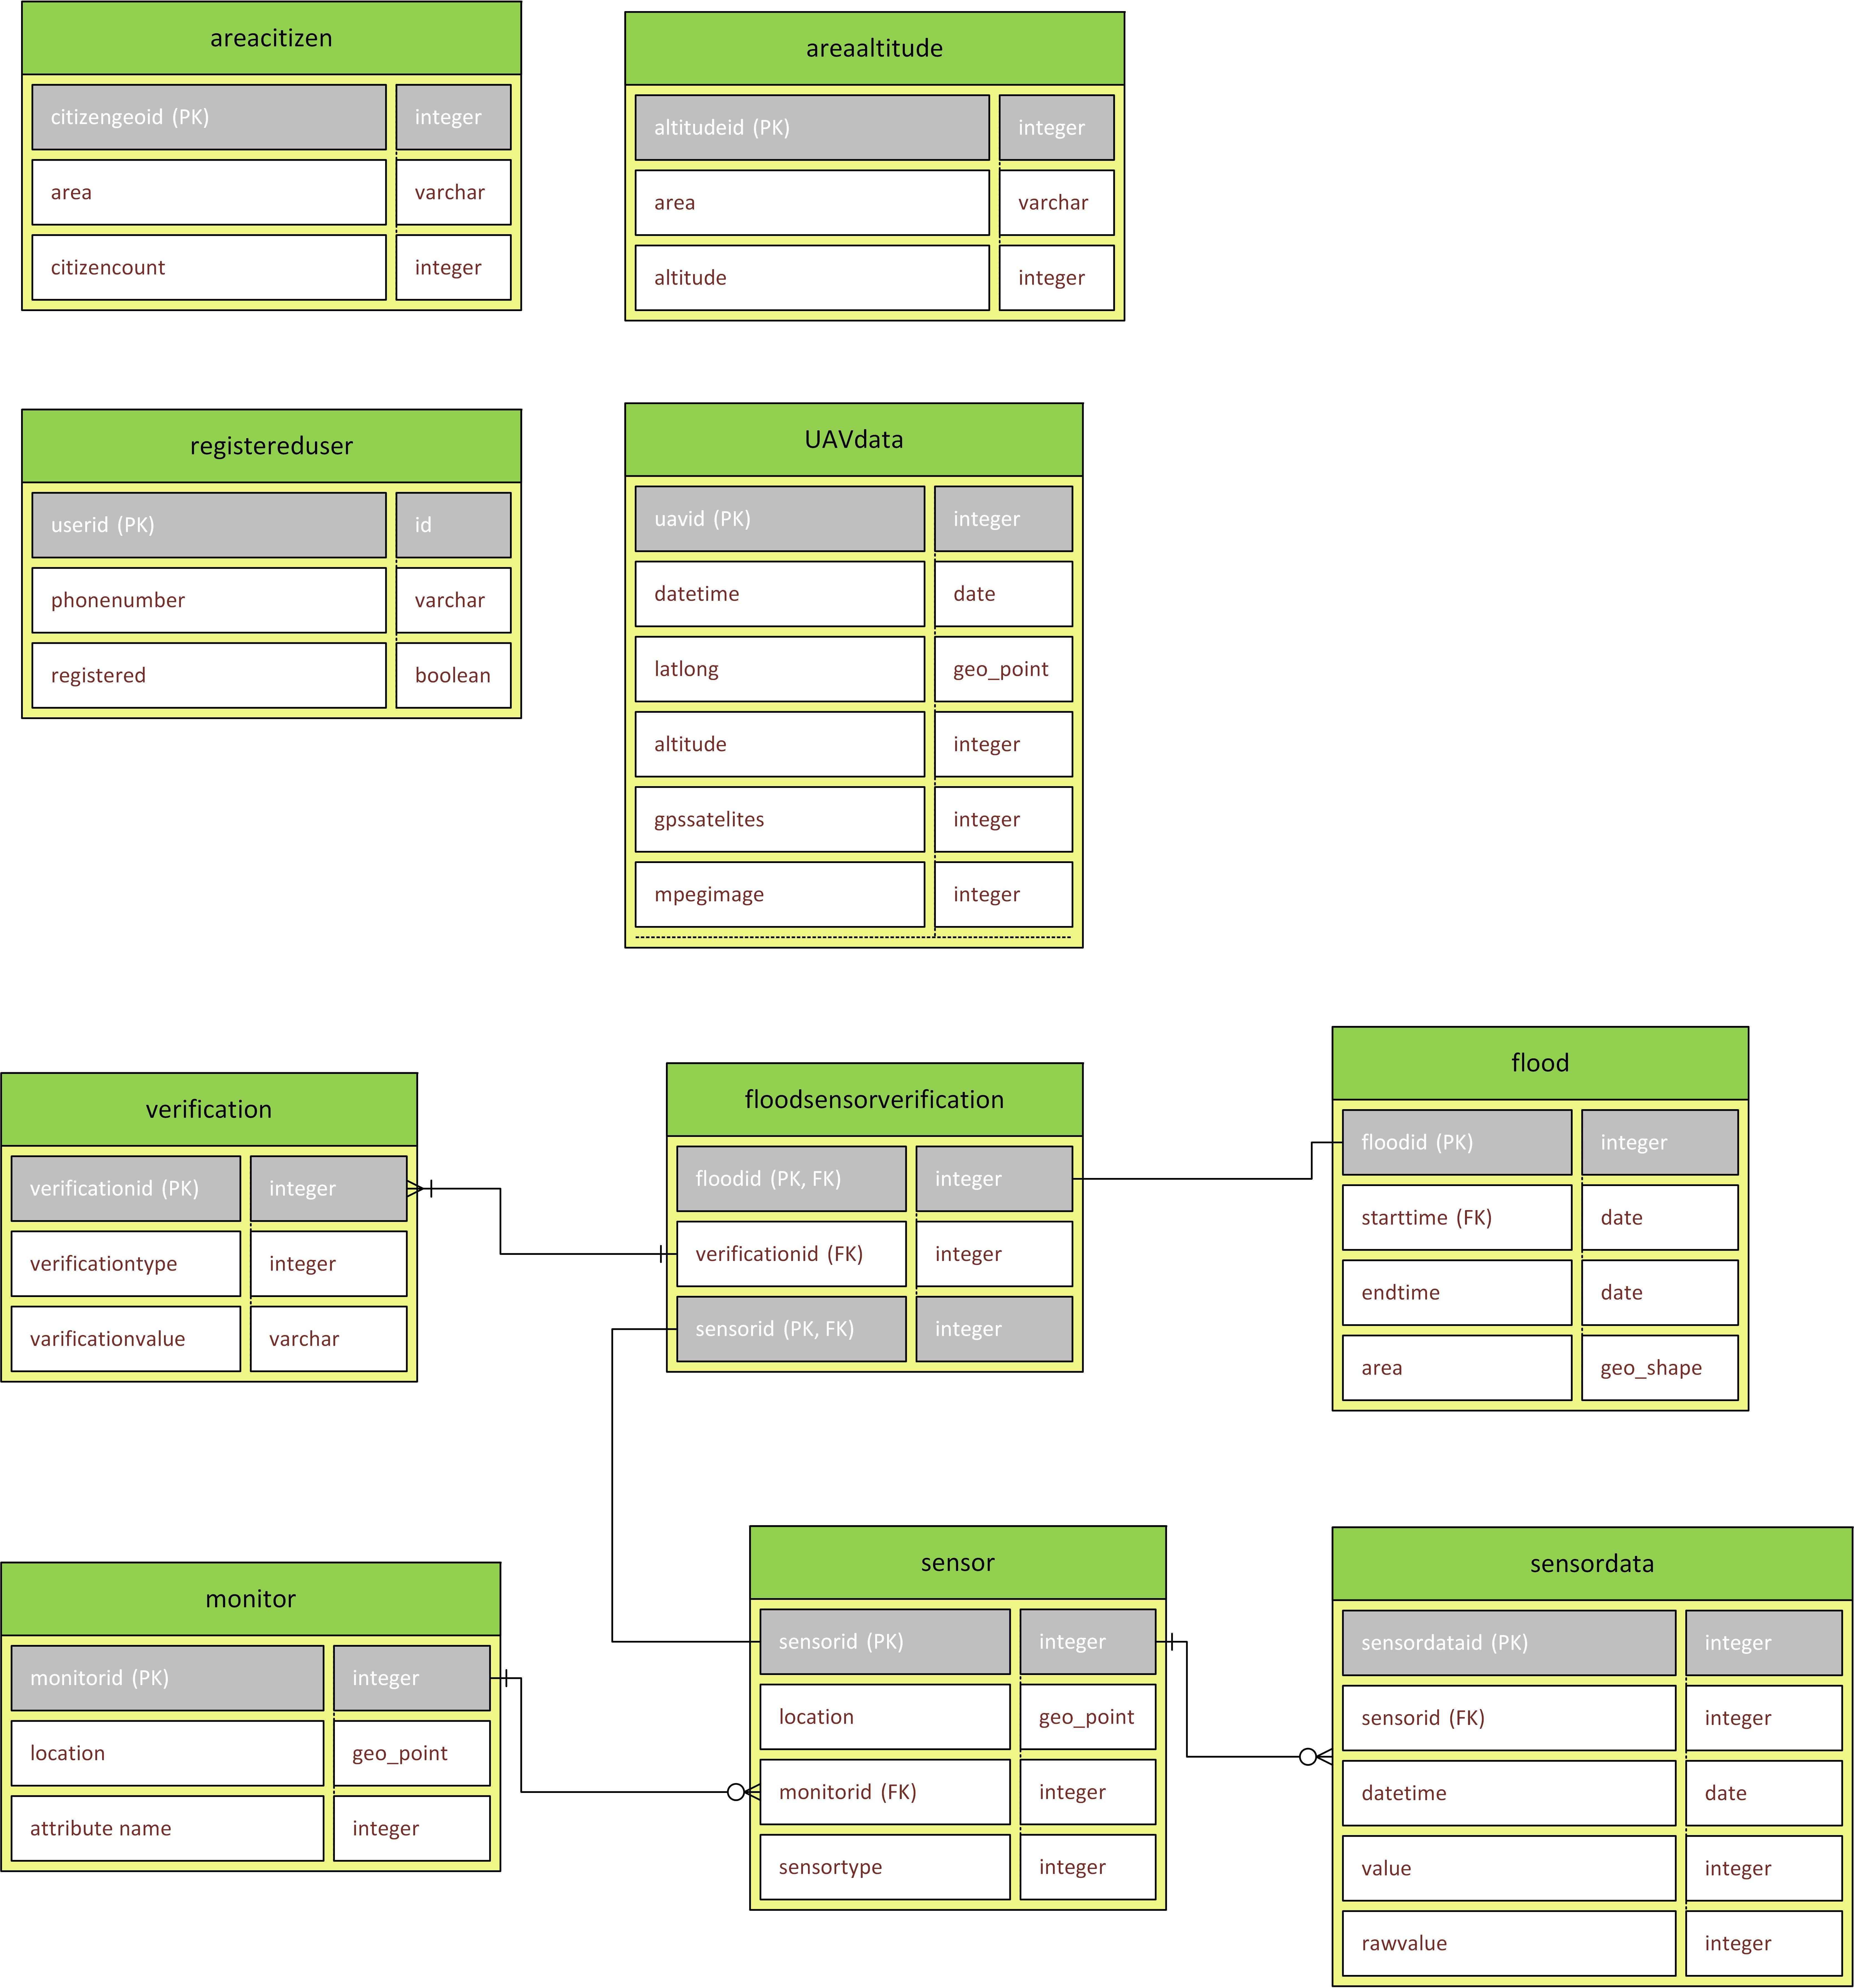
\includegraphics[height=14cm, width=0.9\textwidth]{{\viewimages/database}.jpg}
		\caption{Database diagram}
		\label{fig:database}
	\end{figure}

	% \afterpage{
	\begin{landscape}
	\section{Activity diagram}
	\begin{figure}[H]
		\centering
		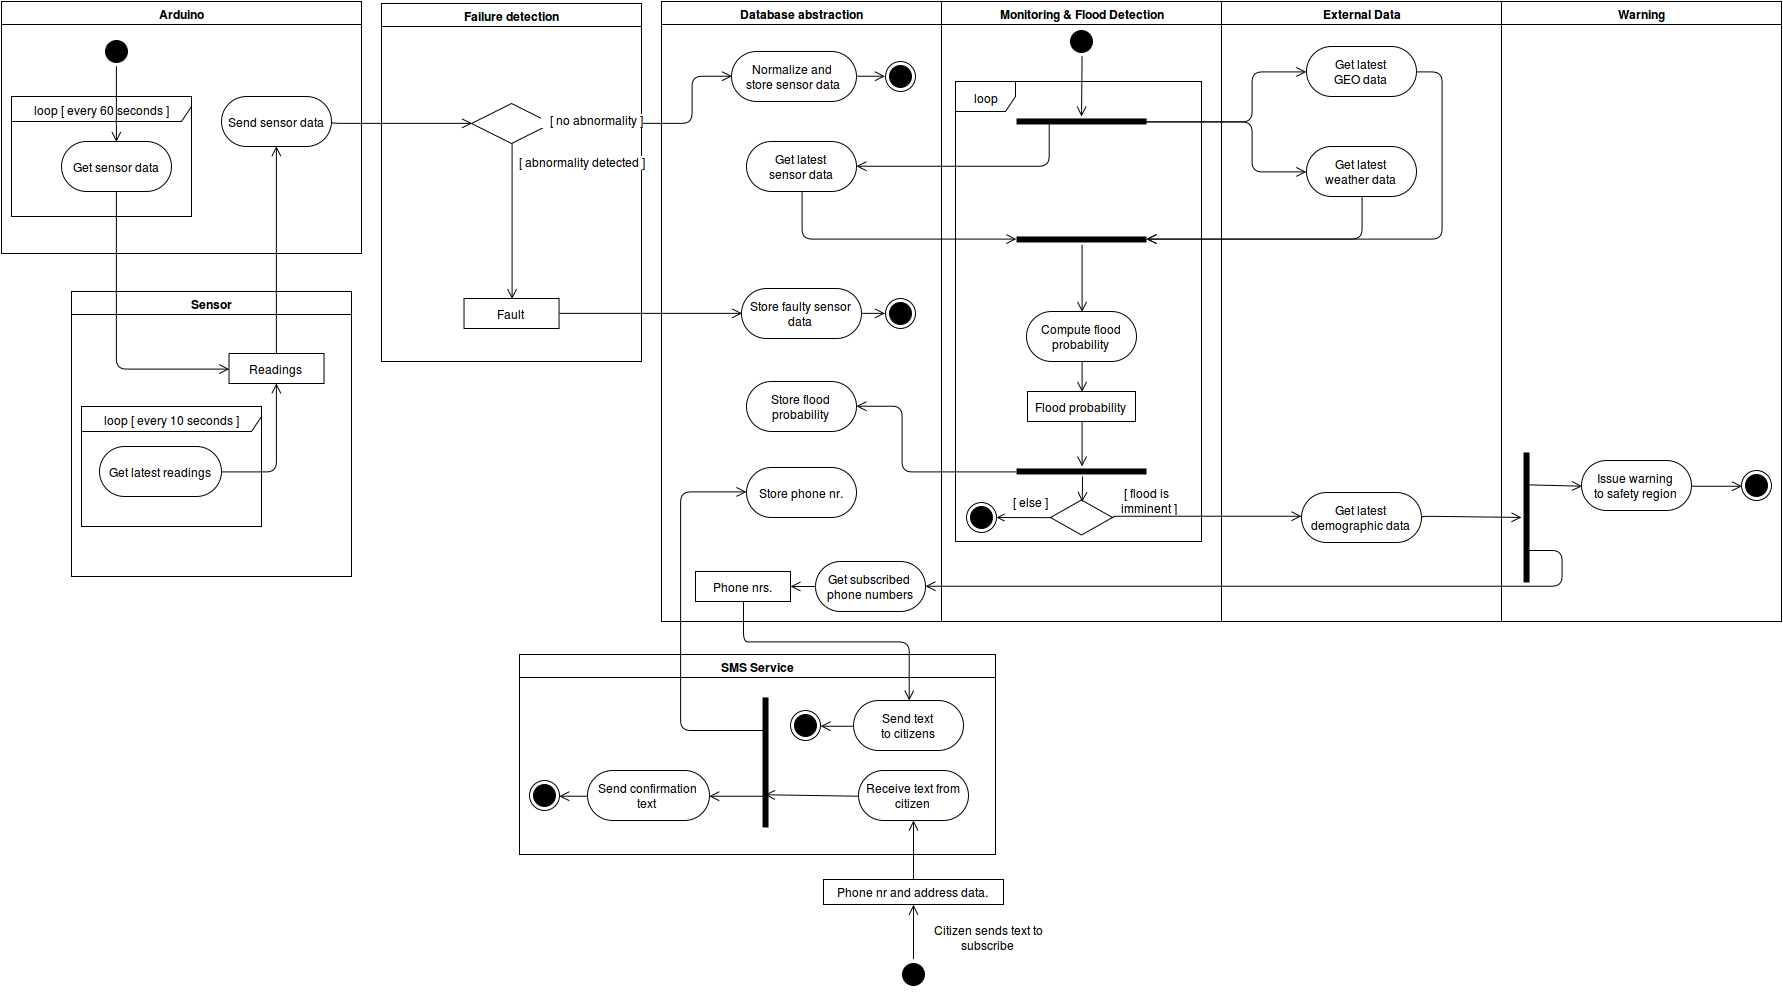
\includegraphics[keepaspectratio=true,width=1.0\textwidth]{{\viewimages/activity_monitoring}.png}
		\caption{An activity diagram of the flood monitoring process}
		\label{fig:activity-monitoring}
	\end{figure}
	% \end{landscape}
	% }
	
	% \afterpage{
	% \begin{landscape}
	\section{Deployment diagram}
	\begin{figure}[H]
		\centering
		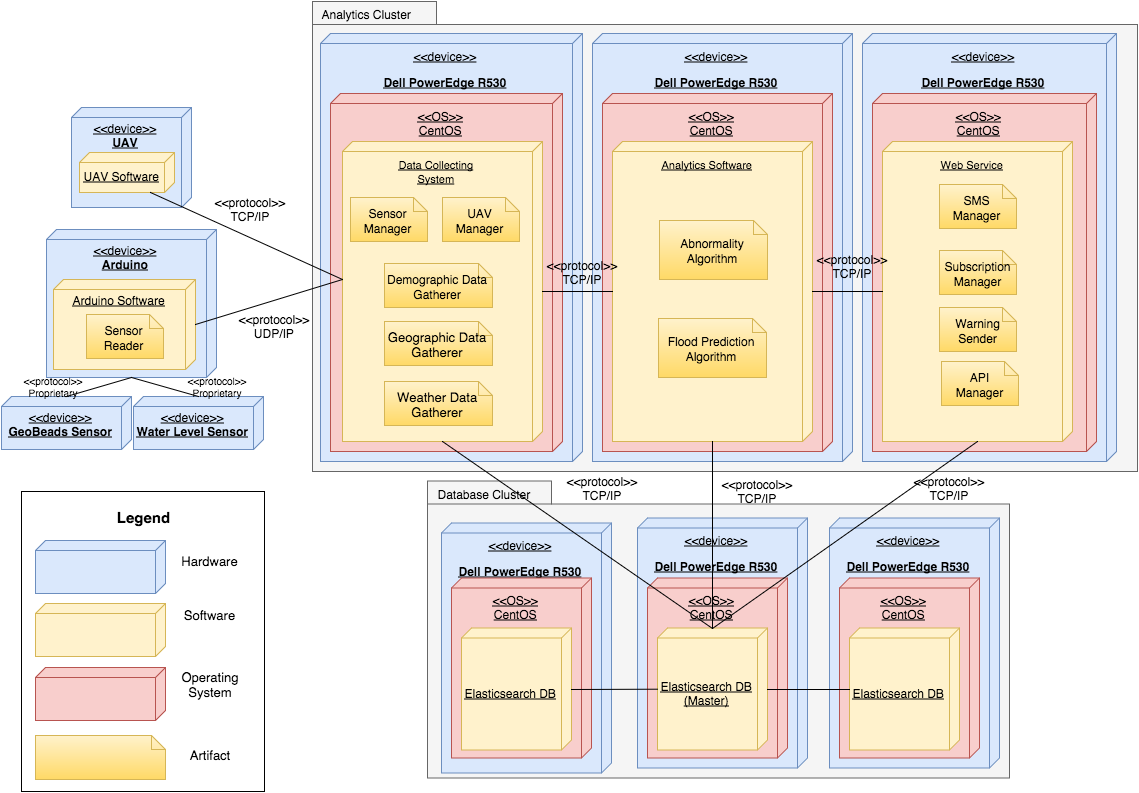
\includegraphics[keepaspectratio=true,width=0.8\textwidth]{{\viewimages/deployment-view}.png}
		\caption{Deployment diagram}
		\label{fig:deployment-diagram}
	\end{figure}
	\end{landscape}
	% }\clearpage

\chapter{Requirements evaluation}
	\label{append:reqeval}
	
	\section{Functional requirements}
		%!TEX root = ../report.tex

%############################################################
%## FUNCTIONAL 
%############################################################

\subsection{Functional requirements evaluation}

\begin{longtable}{llllL{\tw{0.1}}L{\tw{0.4}}}
    \bo{Nr.} & \bo{Priority} & \bo{Fulfilled} & \bo{Decision} & \bo{Chapter} & \bo{Remarks} \\ \toprule \endhead

    %		INTR-1 & Must     & Yes      &~\ref{subsec:external-system} & Fulfilled by using several weather forecast API providers.       \\ \midrule \midrule
    %The system is able to receive input from water level sensors.
    ~\ref{fr:receive-waterlevel} 
    & Must     
    & Yes
    & ~\ref{hw:1}, ~\ref{hw:2}, ~\ref{hw:3} 
    & ~\ref{sec:hardware-overview},~\ref{subsubsec:components}
    ,~\ref{subsec:logicalview} 
    & Fulfilled by the system providing a REST server the arduino sensor systems can use to post the sensor data to. \\ \midrule

    %The system is able to receive input from the dike sensors.
    ~\ref{fr:receive-pressure}
    & Must
    & Yes
    & ~\ref{hw:2}
    &~\ref{sec:hardware-decisions} ~\ref{hw:2}
    & Fulfilled by having arduino systems sent the dike sensor values over a cabled network to the central system's REST server \\ \midrule

    %The system is able to perform an analysis for the parameters of the dike sensors based on the input from the dike sensors.
    %TODO This has to be explained better i guess.
    ~\ref{fr:analyze-pressure}  
    & Must     
    & Yes        
    & ~\ref{hw:1}
    & ~\ref{subsec:logicalview}, ~\ref{subsec:view-process} 
    & Fulfilled, algorithm uses paramaters of dike sensors. \\ \midrule

    %FR-5 Must The system can store the sensor data.
    ~\ref{fr:store-sensordata}  
    & Must     
    & Yes        
    & ~\ref{dec:6}
    & ~\ref{sec:hardware-overview}, ~\ref{subsec:implementview}, ~\ref{subsec:databaseview}
    & Fulfilled by using an ElasticSearch database that is capable of storing all the data needed.\\ \midrule 

    ~\ref{fr:retrieve-sensordata}
    & Must
    & Yes
    & ~\ref{dec:6}
    & ~\ref{subsec:implementview}, ~\ref{subsec:databaseview}
    &Fulfilled by using an Elasticsearch database that is very robust, high available and scalable. Thereby enhancing the ability to store and receive data at all times. \\ \midrule

    %		%The system retrieves weather forecasting data from weather forecasting services,
    %which consists of predictions about the precipitation, wind data and tide information.
    %This is used by the system to help in determining when a flood becomes imminent
    ~\ref{fr:receive-weather}
    & Must
    & Yes
    & 
    &~\ref{subsec:external-system}
    & Fulfilled by the system contacting several API's to base the decisions on. \\ \midrule 

    %The system is able to detect when a flood is imminent by combining the retrieved
    %sensor data and weather forecasting data.
    ~\ref{fr:detect-flood}
    & Must
    & Yes
    &
    &~\ref{subsec:logicalview}, ~\ref{subsubsec:proc-floodmonitor}
    & Fulfilled by the system using Longitudinal Data Analysis to correlate the sensor data with the forecast data \\ \midrule 

    %		%The system retrieves geographic information, consisting of road data, terrain height
    %data and demographic data (number of civilians living in affected area) from an
    %external API.
    ~\ref{fr:receive-geographic}
    & Must
    & Yes
    &
    &~\ref{subsec:external-system}
    & Fulfilled by the system contacting an external GEO API over TCP/IP\\ \midrule

    %		%The system computes the area affected by a flood, in zones of 5 by 5 km, by using the
    %location data of the sensors and geographic information.
    ~\ref{fr:compute-area}
    & Must
    & Yes
    & ~\ref{dec:6}
    & ~\ref{subsec:database-data},~\ref{subsec:external-system}
    & Fulfilled by the system storing the geographical data in an ElasticSearch database, capable of performing queries to get the specified area \\ \midrule 

    %		%The system is able to perform an analysis, resulting in an estimated expected water
    %level for areas which are affected by a flood, based on the water level sensor data,
    %geographic data and weather forecast information.
    ~\ref{fr:analyze-waterlevel}
    & Must
    & Yes
    &
    &~\ref{sec:elaboratedmodel} ~\ref{subsec:logicalview}
    & Fulfilled by using several different external API's for additional information together with a correlation algorithm and other analysis algorithms \\ \midrule 

    %The system estimates how the water level in the areas affected by the flood will %develop for every hour, up to 12 hours in the future.
    ~\ref{fr:estimate-waterlevel}
    & Should
    & Yes
    &
    & ~\ref{subsec:logicalview}
    & Fulfilled by having the system multiple prediction algorithms to analyze the flood data\\ \midrule 

    %The system can compute the number of civilians living in the areas affected by the flood.
    %TODO: Still no idea what those APIs actually give. 
    ~\ref{fr:compute-nrcivilians}
    & Should
    & Yes
    &
    & ~\ref{subsec:external-system}
    & Fulfilled by letting the system obtain the geo information of the civilians from an external API. Then letting the system store this geo data in the ElasticSearch database, capable of executing complex geo queries. \\ \midrule

    %When a flood is imminent, the system sends a warning to the safety region, containing information about the flood: the area affected by the flood, the expected water level in those areas, how the water level will develop in the coming hours and the number of civilians living in the affected area.
    %TODO explain better in ch7?
    ~\ref{fr:warn-safetyregion}
    & Must
    & Yes
    & ~
    & ~\ref{sec:system-context}, ~\ref{subsec:logicalview}, ~\ref{subsubsec:components}, ~\ref{subsec:view-process}
    & Fulfilled by invoking the emergency room API with a message containing data gathered from the sensor data analysis that led to this warning.\\ \midrule 

    %		\frReqRow{citizens-subscribe}{Must}
    %		{ Citizens are able to subscribe to flood warnings about imminent floods. }	
    ~\ref{fr:citizens-subscribe}
    & Must
    & Yes
    & ~
    & ~\ref{subsec:external-system}, ~\ref{subsec:logicalview}
    & Fulfilled by using an external SMS service provider and providing an API that allows user registration\\ \midrule

    %		\frReqRow{warn-citizens}{Must}
    %		{ Citizens who are subscribed for flood warnings are warned about imminent floods by text message. }
    ~\ref{fr:warn-citizens}
    & Must
    & Yes
    & ~
    & ~\ref{subsec:system-alter}
    & Fulfilled by sending the warning message to the external SMS service provider,  who then distributes it\\ \midrule 

    %		\frReqRow{detect-faultysensor}{Must}
    %		{ The system can detect a faulty sensor, either when the sensor raises an error or when the data from the sensor is inconsistent with other sensor data. }

    %TODO add references:
    %TODO not explained good enough
    ~\ref{fr:detect-faultysensor}
    & Must
    & Yes
    & ~
    & ~\ref{subsec:logicalview}
    & Fulfilled by using algorithms to detect abnormalities and then verifying the abnormalities using the other sensors and algorithms\\ \midrule 

    %TODO way to little in the doc about this
    %		\frReqRow{controlpanel}{Must}
    %		{ There is a control panel, where maintainers of the system have access to. } 
    ~\ref{fr:controlpanel}
    & Must
    & Yes
    & ~
    & ~\ref{subsec:view-process}
    & Fulfilled by allowing maintainers to visit a control panel site that uses the REST interface. \\ \midrule 

    %TODO This control panel is not enough described (and do we still use it?)
    %		\frReqRow{report-faultysensors}{Must}
    %		{ The system reports faulty sensors, so they can be viewed in the control panel. }
    ~\ref{fr:report-faultysensors}
    & Must
    & Yes
    & ~
    & ~\ref{subsec:view-process}
    & Fulfilled by storing abnormal sensor data in a different way in the database, allowing the control panel to distinguishes the faulty sensors \\ \midrule 

    %		\frReqRow{controlpanel-warnings}{Must}
    %		{ Warnings of the system can be viewed in the control panel.}
    ~\ref{fr:controlpanel-warnings}
    & Must
    & Yes
    & ~
    & ~\ref{subsec:view-process}
    & Fulfilled by providing a control panel site the maintainers can visit that shows the warnings that the algorithms stored in the database. \\ \midrule 

    %		\frReqRow{controlpanel-errors}{Must}
    %		{ Errors of the system can be viewed in the control panel. }
    ~\ref{fr:controlpanel-errors}
    & Must
    & Yes
    & 
    & ~\ref{subsec:view-process}
    & Fulfilled by providing a control panel site the maintainers can visit that shows the errors that the algorithms stored in the database. \\ \midrule 

    %		\frReqRow{controlpanel-sensors}{Must}
    %		{ The readings of the sensors can be viewed in the control panel. }
    ~\ref{fr:controlpanel-sensors}
    & Must
    & Yes
    & ~
    & ~\ref{subsec:view-process}
    & Fulfilled by providing a control panel site that uses the REST API to get and display the sensor data.\\ \midrule 

    %TODO not explained
    %		Joris: The backups are kind of created by having redundancy
    %		\frReqRow{make-backups}{Must}
    %		{ The system can make backups of its data (configuration data etc.). }
    ~\ref{fr:make-backups}
    & Must
    & Yes
    & ~\ref{dec:7}
    & 
    & Fulfilled by using CentOS as an operating system. This allows the system to be backed up in various ways.\\ \midrule 

    %		\frReqRow{store-backups}{Must}
    %		{ The system can store created backups on a remote location.}
    ~\ref{fr:store-backups}
    & Must
    & Yes
    & ~\ref{dec:7}
    & 
    & Fulfilled by creating backups using rsync \\ \midrule 

    %		\frReqRow{retrieve-backups}{Must}
    %		{ The system can retrieve the backups it previously created.}
    ~\ref{fr:retrieve-backups}
    & Must
    & Yes
    & ~\ref{dec:7}
    & ~
    & Fulfilled by using rsync to backup the system to a accessible location, allowing the system to retrieve the backups\\ \midrule 

    %		\frReqRow{restore-backups}{Must}
    %		{ The system can restore the backups it previously created after retrieving them. }
    ~\ref{fr:restore-backups}
    & Must
    & Yes
    & ~\ref{dec:7}
    & ~
    & Fulfilled by letting the system rsync the backup into the current running system.\\ \midrule 

    %		\frReqRow{expose-api}{Must}
    %		{ The system exposes an API, allowing third parties to develop applications for guidance of the citizens during a flood. }
    ~\ref{fr:expose-api}
    & Must
    & Yes
    & ~\ref{sec:system-context}
    & ~\ref{sec:elaboratedmodel}, ~\ref{subsec:logicalview}, ~\ref{sec:archvision}, ~\ref{subsec:implementview}
    & Fulfilled by hosting a REST sever API\\ \midrule 

    %TODO 	Can it?
    %		\frReqRow{detect-extremephenomena}{Could}
    %		{ The system is able to detect extreme weather phenomena, like storms etc. }
%    ~\ref{fr:detect-extremephenomena}
%    & Could
%    & Partially
%    & ~
%    & ~ 
%    & Partially fulfilled by gathering information from various external weather API's in combination with using a correlation analysis between the sensor values and the external weather data.\\ \midrule

    %TODO explain what algorithms are used?
    %		\frReqRow{uav}{Should}
    %		{ The system processes and stores data collected using a UAV. }	
    ~\ref{fr:uav}
    & Should
    & Yes
    & ~\ref{hw:4}
    & ~\ref{subsec:databaseview}
    & Fulfilled by having a database capable of storing images and geo information\\ \midrule		

    \caption{Evaluation of functional-requirements}
    \label{table:eval-functional-requirements}
\end{longtable}
%\end{longtable}
%\end{adjustbox}

	\section{Non-functional requirements}
		%!TEX root = ../report.tex
%############################################################
%## Commercial non-functional 
%############################################################

\subsection{Commercial non-functional requirements}

\begin{longtable}{llllL{\tw{0.1}}L{\tw{0.4}}}
    \bo{Nr.} & \bo{Priority} & \bo{Fulfilled} & \bo{Decision} & \bo{Chapter} & \bo{Remarks} \\ \toprule \endhead
	
    % %format:
    % ~\ref{} %nr
    % & %priority
    % & %fulfilled
    % & %Decision
    % & %Chapter
    % & %Remarks
    % \\ \midrule

    %\reqRow{CNFR}{affordable}{Must}{The system is affordable. The initial price of the system is lower than 70\%\ of the competitors price in the same market.}
    ~\ref{CNFR:affordable} %nr
    & Must
    & Unknown
    & ~
    & ~
    & Expected. However, the difference in the features offered by our system and the system of the closest competitors makes this requirement hard to verify.
    \\ \midrule

    %\reqRow{CNFR}{lifetime}{Must}{The expected lifetime of the sensors should be at least three years.}
    ~\ref{CNFR:lifetime} %nr
    & Must
    & Yes
    & ~
    & \ref{sec:hardware-description}
    & Fulfilled, the sensors have long lifetime.
    \\ \midrule

    %\reqRow{CNFR}{extendable}{Must}{The system is extendable. At least four updates/versions of the system will be released.}   
    ~\ref{CNFR:extendable} %nr
    & Must
    & Yes
    & ~
    & \ref{sec:evolution-requirements}, \ref{sec:version}
    & Fulfilled, some evolutions are planned.
    \\ \midrule

%    \caption{Evaluation of non-functional commercial requirements} 
%    \label{table:eval-commercialNF-requirements}\\
\end{longtable}

\subsection{Technical non-functional(NF) requirements}
This subsection elaborates about technical non-functional requirements that contain reliability, availability, resilience, performance, interoperability, security, and scalability.

\subsubsection{Reliability}

\begin{longtable}{llllL{\tw{0.1}}L{\tw{0.4}}}
    \bo{Nr.} & \bo{Priority} & \bo{Fulfilled} & \bo{Decision} & \bo{Chapter} & \bo{Remarks} \\ \toprule \endhead

    % %format:
    % ~\ref{} %nr
    % & %priority
    % & %fulfilled
    % & %Decision
    % & %Chapter
    % & %Remarks
    % \\ \midrule
    
    ~\ref{REL:sensors=reachserver} %nr
    & Must
    & Yes
    & ~
    & \ref{sec:hardware-description}
    & Fulfilled, TCP/IP connection will guarantee that data can reach the central server in 99.9\% of all cases.
    \\ \midrule

    ~\ref{REL:sensor-incorrectvalues} %nr
    & Must
    & Yes
    & ~
    & \ref{subsec:logicalview}, \ref{subsec:deploymentview}
    & Fulfilled, Sensor Manager and Abnormality algorithm will check for incorrect values.
    \\ \midrule

    ~\ref{REL:falsenegative} %nr
    & Must
    & Yes
    & ~
    & \ref{subsec:logicalview}
    & Fulfilled, algorithm guarantees that the result is always correct (no false negative).
    \\ \midrule

    ~\ref{REL:falsepositive} %nr
    & Must
    & Yes
    & ~
    & \ref{table:uc-determine-flood-probability}
    & Fulfilled, UAV will make sure false positive will not happen.
    \\ \midrule

%	\caption{Evaluation of non-functional reliability requirements}
%    \label{table:eval-technical-nf}\\
\end{longtable}


\subsubsection{Availability}
\begin{longtable}{llllL{\tw{0.1}}L{\tw{0.4}}}
    \bo{Nr.} & \bo{Priority} & \bo{Fulfilled} & \bo{Decision} & \bo{Chapter} & \bo{Remarks} \\ \toprule \endhead

    % %format:
    % ~\ref{} %nr
    % & %priority
    % & %fulfilled
    % & %Decision
    % & %Chapter
    % & %Remarks
    % \\ \midrule

    \ref{AVA:uptime} %nr
    & Must
    & Yes
    & ~
    & \ref{subsec:availability}
    & Fulfilled, the SFM will not be down for more than 2 hours per month.
    \\ \midrule

    \ref{AVA:downtime} %nr
    & Must
    & Yes
    & ~
    & \ref{sec:hardware-overview}
    & Fulfilled, the SFM has multiple data centers that will minimize downtime.
    \\ \midrule

    \ref{AVA:forecastingservices} %nr
    & Must
    & Yes
    & ~
    &~\ref{subsec:external-system}
    & Fulfilled by the system contacting several API's to base the decisions on.
    \\ \midrule 

%    \caption{Evaluation of non-functional availability requirements} 
%    \label{table:eval-functional-requirements}
\end{longtable}

\subsubsection{Resilience}
\begin{longtable}{llllL{\tw{0.1}}L{\tw{0.4}}}
    \bo{Nr.} & \bo{Priority} & \bo{Fulfilled} & \bo{Decision} & \bo{Chapter} & \bo{Remarks} \\ \toprule \endhead
    
    % %format:
    % ~\ref{} %nr
    % & %priority
    % & %fulfilled
    % & %Decision
    % & %Chapter
    % & %Remarks
    % \\ \midrule

    %\reqRow{RES}{recognizefail}{Must}{The system recognizes failures within half an hour}
    ~\ref{RES:recognizefail} %nr
    & Must
    & Yes
    & ~
    & \ref{subsec:logicalview}
    & Fulfilled, the system recognizes failure in each data reads which means significantly less than half an hour.
    \\ \midrule

    % \reqRow{RES}{failrecover}{Must}{The system recovers from failures without the performance or the functionality of the system being affected.}
    ~\ref{RES:failrecover} %nr
    & Must
    & Yes
    & \ref{hw:5}, \ref{hw:6}
    & \ref{sec:hardware-overview}, \ref{sec:hardware-description}
    & Fulfilled, the servers are replicated thus the system is fault-tolerant.
    \\ \midrule

    % \reqRow{RES}{backup}{Must}{All system data must be backed up every 24 hours.}
    ~\ref{RES:backup} %nr
    & Must
    & Yes
    & ~
    & \ref{subsec:database-data}
    & Fulfilled, the database is replicated which means the data is always backed up.
    \\ \midrule

    % \reqRow{RES}{backuprestore}{Must}{In case of a data loss, the data should be retrieved and restored from a backup within 2 hours.}
    ~\ref{RES:backuprestore} %nr
    & Must
    & Yes
    & ~
    & \ref{subsec:database-data}
    & Fulfilled, the database is redundant which means restoring data takes significantly less than two hours.
    \\ \midrule

    % \reqRow{RES}{backuparea}{Must}{Backup copies are stored in a location which is not in the same area as the system (50 km away).}
    ~\ref{RES:backuparea} %nr
    & Must
    & Yes
    & ~
    & \ref{sec:hardware-overview}, \ref{subsec:database-data}
    & Fulfilled, the SFM has three data centers that are located more than 50km away.
    \\ \midrule

%	\caption{Evaluation of non-functional resilience requirements}
%    \label{table:eval-technical-nf}\\
\end{longtable}

\subsubsection{Performance}
\begin{longtable}{llllL{\tw{0.1}}L{\tw{0.4}}}
	\caption{Evaluation of non-functional performance requirements}
    \label{table:eval-technical-nf}\\

    \bo{Nr.} & \bo{Priority} & \bo{Fulfilled} & \bo{Decision} & \bo{Chapter} & \bo{Remarks} \\ \toprule \endhead

        %	\reqRow{perf}{Must}{Data is transmitted from and to the system with a minimum average speed of 10 megabits per second}
        \ref{perf:transmissionspeed}
        & Must
        & Yes
        & \ref{hw:7}
        & \ref{sec:hardware-decisions}, \ref{sec:hardware-description} 
        & Fulfilled, each components of the system are connected by Gigabit Ethernet. \\ \midrule
        
        %	\reqRow{perf}{Must}{	The data transmission between the sensors and the system is on average at least 10 megabits per second for each sensor.}
        \ref{perf:transpersec} 
        & Must     
        & Yes  
        & \ref{hw:3} 
        & \ref{sec:hardware-decisions} 
        & Fulfilled, Arduinos that are connected to sensors send data in 10 Megabits per second. \\ \midrule
        
        %	\reqRow{perf}{Must}{	The time for the system to compute if there is a flood or not according to a critical level and the data received from the sensors is at most 5 minutes. }
        \ref{perf:timetocompflood} 
        & Must     
        & Yes  
        & ~ 
        & \ref{sec:hardware-description} 
        & Fulfilled, analytics cluster will compute this calculation. \\ \midrule
        
        %	\reqRow{perf}{Must}{ If an imminent flood is detected, the warning text message to citizens arrives in 5 minutes. }
        \ref{perf:wantextimecitizen} 
        & Must     
        & Yes  
        & ~ 
        & \ref{subsec:external-system}, \ref{subsec:logicalview}         
        & Fulfilled, SMS service will make sure the SMS will arrive within 5 minutes. \\ \midrule
        
        %	\reqRow{perf}{Must}{ If an imminent flood is detected, the warning to the emergency room arrives within 1 minute. }
        \ref{perf:warntimetextregion} 
        & Must     
        & Yes  
        & ~ 
        & \ref{subsec:external-system}, \ref{subsec:logicalview}         
        & Fulfilled, TCP/IP connection guarantees that the information will arrive within one minute. \\ \midrule
    \end{longtable}

\subsubsection{Interoperability}

\begin{longtable}{llllL{\tw{0.1}}L{\tw{0.4}}}

%	\caption{Evaluation} of non-functional interoperability requirements}
%    \label{table:eval-technical-nf}
    
    \bo{Nr.} & \bo{Priority} & \bo{Fulfilled} & \bo{Decision} & \bo{Chapter} & \bo{Remarks} \\ \toprule \endhead
		% \reqRow{intr}{Must}{The system is able to retrieve data from different types of water level sensors and dike sensors. Also future versions of the sensors should be supported.}       
        \ref{intr:sensortype} & Must     & Yes      & ~\ref{dec:3} & ~\ref{sec:hardware-overview} & Fulfilled by using GeoBeads and Water level sensor. \\ \midrule
        % \reqRow{intr}{Must}{The system is able to retrieve external data from different weather forecast, demographic and geographic APIs. Also future versions of the APIs should be supported.}
        \ref{intr:forecast} & Must     & Yes      & &~\ref{subsec:external-system} & Fulfilled by using several external API providers.       \\ \midrule
\end{longtable}

\subsubsection{Security}
\begin{longtable}{llllL{\tw{0.1}}L{\tw{0.4}}}
%	\caption{Evaluation of non-functional security requirements}
%    \label{table:eval-technical-nf}
    
        Nr.   & Priority & Fulfilled & Decision & Chapter & Remarks \\ \midrule
        % \reqRow{sec}{Must}{Access to the system is restricted to users, which are authorized and authenticated using a password protected user account.}
        \ref{sec:userpassprotect} & Must     & Yes      & & ~\ref{subsec:system-diagram} & Fulfilled, the user must be authorized to enter the system. \\ \midrule
        
        % \reqRow{sec}{Must}{All communication to, from and within the system is encrypted.}
        \ref{sec:encryptedcomm} & Must     & Yes      & ~\ref{dec:9} & ~\ref{subsec:channels-information-flows} & Fulfilled, by using secure channel. \\ \midrule
        
        % \reqRow{sec}{Must}{User account information is stored encrypted.}
        
        \ref{sec:encryptaccount} & Must     & Yes      & ~\ref{dec:6} & ~\ref{subsec:database-data} & Fulfilled, applied in Elasticsearch DB. \\ \midrule
        
        % \reqRow{sec}{Must}{The system is protected on both the application layer and network layer.}
        
        \ref{sec:networkprotection} & Must     & Yes      & & ~\ref{sec:hardware-overview} & Fulfilled, in the data center level. \\ \midrule
        % \reqRow{sec}{Must}{The system communicates with the sensors via a secure HTTPS connection.}
        
        \ref{sec:https} & Must     & Yes      & ~\ref{dec:9} & ~\ref{sec:hardware-overview} & Fulfilled, by using Arduino to send data. \\ \midrule

\end{longtable}

\subsubsection{Scalability}
\begin{longtable}{llllL{\tw{0.1}}L{\tw{0.4}}}
%	\caption{Evaluation of non-functional scalability requirements}
%    \label{table:eval-technical-nf}\\
        Nr.     & Priority & Fulfilled & Decision & Chapter & Remarks \\ \midrule
        % \reqRow{scale}{Must}{The database and services of the system can scale within 1 hour, when the systems resource usage increases.}
        
        \ref{scale:scaletime} & Must     & Yes      & ~\ref{dec:6} & ~\ref{subsec:database-data} & Fulfilled by adapting Elasticsearch. \\ \midrule
        % \reqRow{scale}{Must}{The system is configurable to run in different areas and with different sensors.}
        
        \ref{scale:areas} & Must     & Yes      & & ~\ref{sec:hardware-overview} & Fulfilled by adapting multiple data centers and multiple sensor type. \\ \midrule
        
        % \reqRow{scale}{Must}{The system maintains the performance requirements when the number of sensors is increased and the data from sensors is expanded.}
        
        \ref{scale:moresensors} & Must     & Unknown  & & -         & Expected, not yet tested. \\ \midrule


\end{longtable}



	%!TEX root = ../report.tex
\chapter{Time Tracking}
\label{App: Time Tracking}

%\section{Week #}
%\begin{tabular}{p{0.2\textwidth} p{0.7\textwidth} p{0.1\textwidth}}
%    \textbf{Person} & \textbf{Task} & \textbf{Hours} \\ \midrule
%	Eedema &  &  \\ \midrule
%	Putra &  &  \\ \midrule
%	Fakambi & & \\ \midrule
%	Schaefers &  & \\ \midrule
%	Brandsma &  & \\ \midrule
%	Menninga &  &  \\ \midrule
%\end{tabular}

\section{Week 1}
\begin{tabular}{L{0.2\textwidth} L{0.7\textwidth} L{0.1\textwidth}}
    \textbf{Person} & \textbf{Task} & \textbf{Hours} \\ \toprule
	Eedema & Reviewing the document, reading the assignment, initializing requirements, \& installing environment for project & 8 \\ \midrule
	Putra & Initial preparation for the course & 5 \\ \midrule
	Fakambi & Reading the document and assignment, Preparation and drafts with ideas & 5 \\ \midrule
	Schaefers & Setting up the working environment, create the context page and analysis page drafts. Setting up and improving the the document structure. & 8\\ \midrule
	Klinkenberg & & \\ \midrule
	Brandsma & Creating working environment, reading assignment, first draft business part & 8\\ \midrule
	Menninga & Reading assignment, setting up working environment, first non-functional requirements & 5 \\ \bottomrule
\end{tabular}

\section{Week 2}
\begin{tabular}{L{0.2\textwidth} L{0.7\textwidth} L{0.1\textwidth}}
    \textbf{Person} & \textbf{Task} & \textbf{Hours} \\ \toprule
	Eedema & Coaching session, project planning session and work on business information chapters & 9  \\ \midrule
	Putra & Coaching session, project planning session, project meeting, first version of stakeholder part of requirements & 7.5 \\ \midrule
	Fakambi & Coaching session , project meeting, work on Non functional requirements & 7 \\ \midrule
	Schaefers & First coaching session, improved and enhanced the context and business information chapters. Also created a quality attributes prioritization table.& 8 \\ \midrule
	Klinkenberg & Coaching session, meetings, providing feedback on requirements & 5.5\\ \midrule
	Brandsma & First version of use-cases, coaching session, meeting, use-cases, architectural vision & 6.5 \\ \midrule
	Menninga & First version of the functional requirements, coaching session, meeting & 10.25 \\ \bottomrule
\end{tabular}

\section{Week 3}
\begin{tabular}{p{0.2\textwidth} p{0.7\textwidth} p{0.1\textwidth}}
   \textbf{Person} & \textbf{Task} & \textbf{Hours} \\ \midrule
	Eedema &  Coaching, meetings, analysis, business part, reviewing & 14  \\ \midrule
	Putra & Coaching session, meetings, proofread on chapter 1 and 2, revising stakeholders, database decision part of analysis, and preparing \LaTeX{} file for the presentation & 10 \\ \midrule
	Fakambi & Coaching session, meetings, Non functional requirements and Risk assessment & 10.5\\ \midrule
	Schaefers & Coaching session, meetings, reviewing, Business section & 12 \\ \midrule
	Klinkenberg & Coaching session, meetings, technical requirements, analysis, reviewing & 13.5 \\ \midrule
	Brandsma & Coaching session, meeting, architectural vision, use-cases, analysis & 9 \\ \midrule
	Menninga & Coaching session, meetings, updates functional requirements, reviewing entire document, updated assumptions and some improvements to structure of analysis, added decision about type of water level sensor. & 14.0 \\ \midrule
\end{tabular}

\section{Week 4}
\begin{tabular}{p{0.2\textwidth} p{0.7\textwidth} p{0.1\textwidth}}
   \textbf{Person} & \textbf{Task} & \textbf{Hours} \\ \midrule
	Eedema & Coaching session, meetings, business chapter, review 3, presentations, peer review &13  \\ \midrule
	Putra & Coaching session, meetings, presentation prep., improving business rationale, review chapter 2, making draft of chapter 5, 6, and 7 & 14 \\ \midrule
	Fakambi & Coaching session , meetings , Work on and improvements chapter 3.5 to 3.8 & 12 \\ \midrule
	Schaefers & Researched on sensors and other EWS's. Then created the system architecture model diagram and vision diagram for the presentation I had to present in. Created/improved other diagrams. Researched about the costs of these kinds of systems and created/enhanced the business cost section. & 20 \\ \midrule
	Brandsma & Coaching session, meetings , reviewing group 1, architectural vision, use-cases, reviewing, improving chapter 4 & 16.5\\ \midrule
	Menninga & Coaching session, presentation prep., meeting, improvements FR and risks, review ch. 4, improvements to NFR and Risk Assessment & 14.0 \\ \midrule
\end{tabular}

\section{Week 5}
\begin{tabular}{p{0.2\textwidth} p{0.7\textwidth} p{0.1\textwidth}}
    \textbf{Person} & \textbf{Task} & \textbf{Hours} \\ \midrule
	Eedema & Coaching meetings, reviewing, chpt 5  & 13 \\ \midrule
	Putra & Coaching session, meetings, reviewing, working on initial work on chapter hardware, researching on servers, and working on server selection  & 15 \\ \midrule
	Fakambi & Coaching session, meetings, Work on chapter 6 Hardware architecture, drafts, design decision about UAVs & 12.0 \\ \midrule
	Schaefers & Created initial layer diagram, component diagram, sequense diagram and database design diagram. Researched and explained what new database to use.  & 15\\ \midrule
	Brandsma & Coaching session, meetings, chapter 5  & 13 \\ \midrule
	Menninga & Coaching session, meeting Tuesday, lots of improvements to chapter 3, expanding chapter 6 & 15.5 \\ \midrule
\end{tabular}

\section{Week 6}
\begin{tabular}{p{0.2\textwidth} p{0.7\textwidth} p{0.1\textwidth}}
    \textbf{Person} & \textbf{Task} & \textbf{Hours} \\ \midrule
	Eedema & Coaching, meetings, review, system overview, evaluation & 15 \\ \midrule
	Putra & Coaching session, meetings, reviews, hardware overview, deployment view & 13 \\ \midrule
	Fakambi & Coaching session, meetings, Work on chapter 6 Hardware architecture, drafts, design decision about UAVs, draft about chapter 7 & 9 \\ \midrule
	Schaefers & Meetings. Worked on the implementation and logical section of the software chapter. & 13 \\ \midrule
	Brandsma & &  \\ \midrule
	Menninga & Coaching session, meetings, reviews, hardware overview (sensors)/costs, implementation view, process view & 13.0 \\
	\midrule
\end{tabular}
	% %!TEX root = ../report.tex
\chapter{Todo} % (fold)
\label{sec:todo}
\todo[inline]{Create figure with processflow and place it somewhere logical}
% section todo (end)



	
\end{appendices}